%!TEX root = ../thesis.tex

% https://en.wikipedia.org/wiki/Kelly_Johnson_(engineer)
% https://en.wikipedia.org/wiki/KISS_principle
\begin{savequote}[40mm]
	\textbf{K}eep\\
	\textbf{I}t\\
	\textbf{S}imple\\
	\textbf{S}tupid
	\qauthor{Kelly Johnson}
\end{savequote}

\chapter{Proposed solution}\label{chapter:proposed_solution}
	
	\textbf{\textcolor{red}{\hl{// To be completed with one or two phrases}}}

	This chapter contains the technical description of the mesh network developed with the FiPy and communicates using LoRa.
	Such mesh network will be referred as ``\textit{Open LoRa Mesh}''.
	Especially such networks is able to accommodate small messages, such as the ones sent by MegaSense, described in Section~\ref{subsec:megasense}.

	Even though it would have been possible to use a simulator, such as ``\textit{The one}''\footnote{ \url{akeranen.github.io/the-one}}, for demonstrating the usefulness of such network, the final project has been realized with Pycom hardware, discussed in Section~\ref{sec:hardware_solution}.
	
%	The code created for this project is open sourced and available on GitHub\footnote{ \url{www.github.com/cipz/OpenLoRaMesh}}.
%	Such code is better explained later in Section~\ref{sec:software_solution} and its subsections.
	
	\section{Network architecture}\label{sec:architecture}
		
		Before talking about the architecture of the mesh, it is important to understand the one of the MegaSense.
		As can be seen in Figure~\ref{img:megasense_architecture}, since each MegaSense device is made to be carried by a person, devices connect each one to the user's phone.
		The latter then communicates with the MegaSense and, via the application developed by the Computer Science Department at the University of Helsinki, sends the air-quality readings and the GPS location, which has been read by the application from the phone itself, to the servers in the cloud.
		
		Communication between MegaSense and phone is done via BLE, and exchanges data such as sensor readings (like NO2,
		O3, CO, battery percentage, \textit{etc.}) and calibration measurements, in \texttt{JSON} format.
		Thus each device has to be linked to a person's phone, which might enhance the portability of the device, but not its possibility to read data independently if placed in a specific location.
		
		\begin{figure}[h]
			\centering
			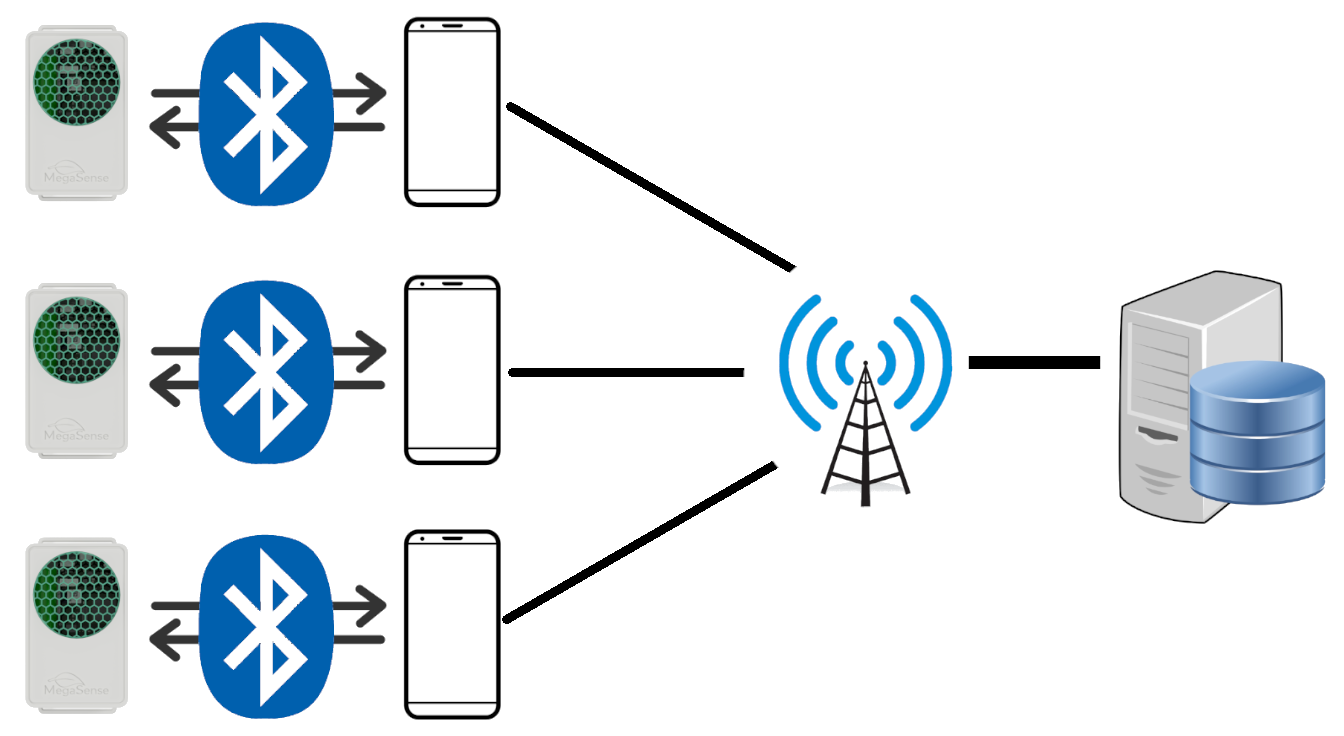
\includegraphics[width=.75\textwidth]{resources/img/chap5/architecture_megasense}
			\caption{MegaSense architecture}
			\label{img:megasense_architecture}
		\end{figure}
	
		One of the goals Open LoRa Mesh tries to achieve, is to give independence to these devices, so that they can communicate one another and allow information to be passed along between nodes without the aid of a user's phone.
	
		This is why the architecture would evolve from the one in Figure~\ref{img:megasense_architecture} to Figure~\ref{img:openmesh_architecture}: the phone is replaced by a FiPy, which also connects to the MegaSense via BLE, and sends the data acquired from the sensors in the network.
		Nodes communicate with each other via LoRa, detailed in Section~\ref{subsec:lora_lorawan}, and exchange data using mainly \textit{LoRaCTP}, described in Section~\ref{subsec:loractp}.
		
		\begin{figure}[h]
			\centering
			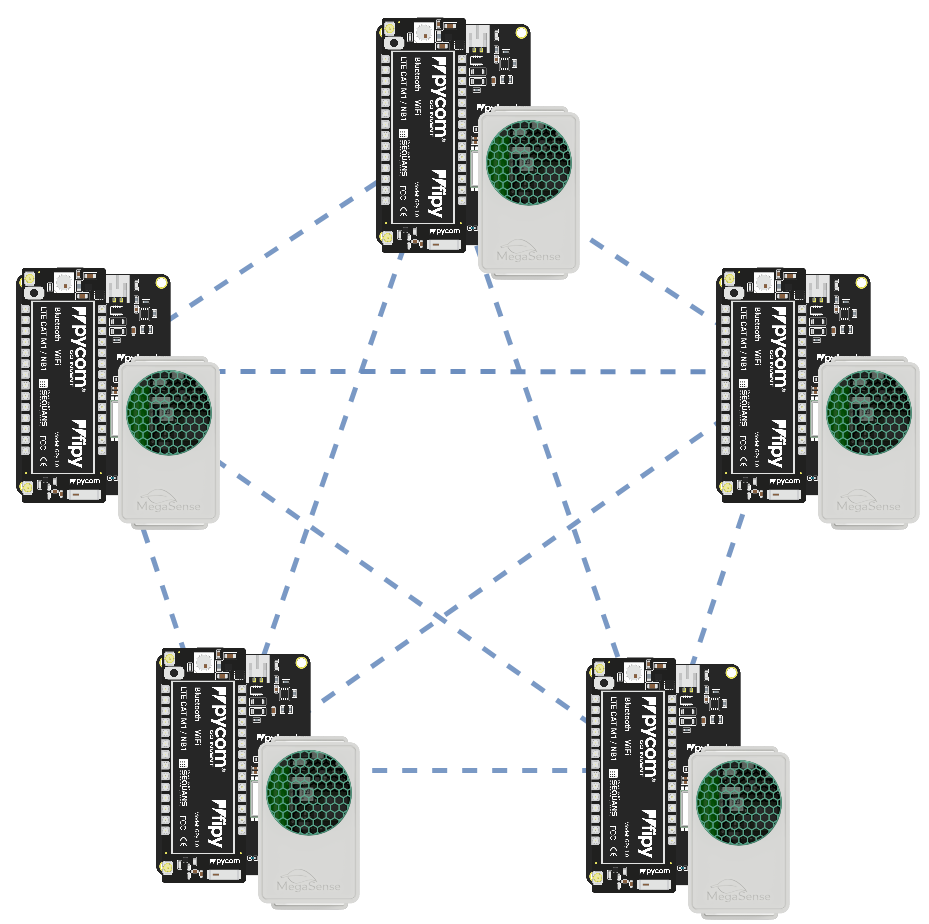
\includegraphics[width=.7\textwidth]{resources/img/chap5/mesh-architecture-1}
			\caption{Open LoRa Mesh architecture}
			\label{img:openmesh_architecture}
		\end{figure}
		
		Each FiPy board represents a node on the network, which in this case is a ``\textit{Flat Wireless Mesh}'', where each node acts both as data provider and as data forwarder.
		Although simple, such network architecture is well known from the previously mentioned, Section~\ref{sec:scalability}, Gupta and Kumar \cite{825799}.
		Besides not scaling well and having the potential to put very high resource constraints, ``\textit{addressing schemes and service discovery would prove to be a major bottleneck against scalability}'' \cite{92000412}.

	\section{Open LoRa Mesh Hardware}\label{sec:hardware_solution}
	
		For the development of Open LoRa Mesh, the chosen hardware to replace the phone in the original MegaSense architecture is composed by Pycom's FiPy microcontrollers, along with its shields, like the PyTrack and the PySense.
		A prototype of the MegaSense device was also given from the developers of the project in order to test the connectivity with the Pycom boards and test its capacity to send and receive data from other nodes in the network.
		All devices can be seen together in Figure~\ref{img:irl_picture_1}.
		
		\begin{figure}[h]
			\centering
			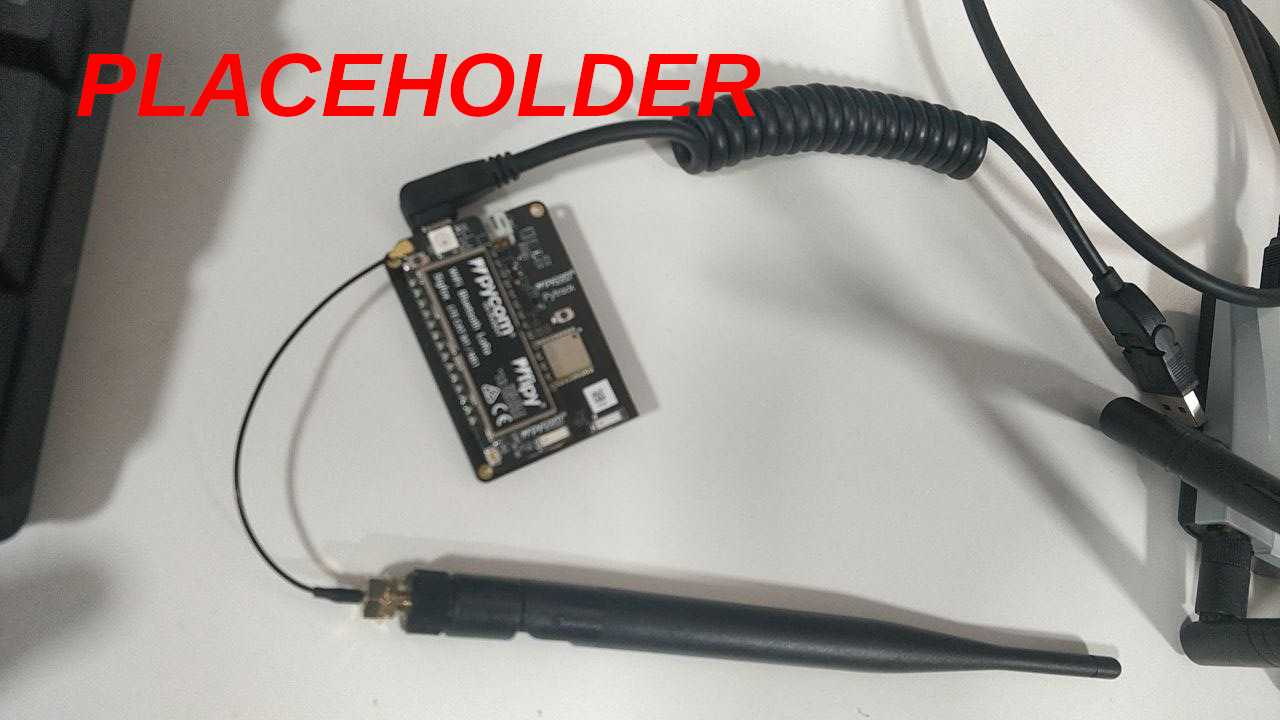
\includegraphics[width=\textwidth]{resources/img/chap5/mesh-irl-picture}
			\caption{FiPy with PyTrack, LoRa antenna, GPS antenna and MegaSense prototype}
			\label{img:irl_picture_1}
		\end{figure}
		
		Although the expansion board is important, the FiPy is the one that contains all the chips that allow connectivity, as said in Section~\ref{sec:pycom}.
		After an initial evaluation on the requirements necessary in creating a network for exchanging messages among air quality sensing devices, Pycom's boards have come first considering the numerous possibilities it allows for prototyping.
		
		The exact hardware with which this project has been completed is: four FiPy boards, one PyTrack 2X, one PyTrack, two PySense shields and one MegaSense prototype, Figure~\ref{img:megasense_picture}.
		Pycom boards do not have a USB connection directly on them, so they can be programmed either using a shield or via an UART (Universal Asynchronous Receiver-Transmitter) to USB.
		
		Alternative microcontrollers, such as the Raspberry Pi Pico, Raspberry Pi 4, Arduino Nano 33 BLE Sense, and ESP32 boards have been discard given either their excessive power or their need for multiple expansion shields.
				
	\section{Open LoRa Mesh Software}\label{sec:software_solution}
	
		While the Arduino's C++ dialect divides the code in two main functions, the \texttt{setup()} and \texttt{loop()}, as mentioned in Chapter~\ref{chapter:technologies}, the Pycom boards use two files to separate an initial bootstrap of the board and a main section of the code.
		These two special files are called \texttt{boot.py} and \texttt{main.py} respectively.
		
		The following section explains the addressing scheme in LoRa, which is important to understand.
		Afterwards, the algorithms made for this project are delineated and it is shown how they have been implemented.
		
		The FiPy boards have been programmed using Micropython, and the firmware flashed on the boards, at the time of writing, is \texttt{v1.16.5}.
		
		\subsection{LoRa addressing scheme}\label{subsec:lora_addressing}
		
			\textbf{\textcolor{red}{\hl{// To be completed}}}
		
			% Hardware Addressing Schemes
		
		
			%calcolare transmission times
		
%		\newpage\phantom{blabla}
%		\newpage\phantom{blabla}
%		\newpage\phantom{blabla}
%		\newpage\phantom{blabla}	
		
		\subsection{Algorithms}\label{subsec:algorithms}
	
			% DRAWING AUTOMATA
			% https://latexdraw.com/automata-diagrams-in-latex/
			% https://hayesall.com/blog/latex-automata/
			
			% DRAWING FLOWCHART
			% https://www.overleaf.com/learn/latex/LaTeX_Graphics_using_TikZ%3A_A_Tutorial_for_Beginners_(Part_3)%E2%80%94Creating_Flowcharts

			This section shows in depth how the software works: for each significant building block of the code there are flowcharts and finite-state automata (or FSA).
			The flowcharts describe the algorithms and show what functions are called, while finite-state machines show what states the devices can be in and how they arrive in such states.
			% Note: automata is plural
			For a graphical reason, each state of the following automata is abbreviated, and the full state is described in a table underneath it.
			
			Such vision should allow to understand the system from a broader point of view to a more detailed one, where every function is analyzed.
			
			\subsubsection{Overview of the whole system}
			
				As previously said, the FiPy is divided in two files, \texttt{boot.py} and \texttt{main.py}.
				
%				\begin{figure}[h]
%					\centering
%					\begin{tikzpicture}[shorten >=1pt,node distance=2cm,on grid,auto]
%					
%					% Help grid
%					% \draw [help lines] (-1,1) grid (6,-6);
%					
%					\tikzstyle{every state}=[fill={rgb:black,1;white,5}]
%					
%					
%					\node[state, initial]  			(s_0)                 	{$s_0$}; % START
%					\node[state] 					(s_1)	[right of=s_0]	{$s_1$}; % BOOT
%					\node[state, accepting]			(s_2) 	[above right of=s_1]	{$s_2$}; % MAIN LOOP
%					\node[state, accepting]			(s_3) 	[below right of=s_1]	{$s_3$}; % LISTENER LOOP
%					
%					\path[->]
%					(s_0) edge node {} (s_1)
%					(s_1) edge node {} (s_2)
%					(s_3) edge node {} (s_1)
%					(s_2) edge [loop right] node {} ()
%					(s_3) edge [loop right] node {} ();
%					
%					\end{tikzpicture}
%					\caption{FSA for the overview of the whole system}
%					\label{img:fsa_overview}
%				\end{figure}
%			
%				\begin{table}[h]
%					\begin{center}
%						\begin{tabularx}{0.85\textwidth}{@{}|Y|Y|Y|@{}} 
%							\hline
%							State abbreviation & Full state name & State description \\\hline
%							$start$ && \\\hline
%							$s_{0}$ && \\\hline
%							$s_{1}$ && \\\hline
%							$s_{2}$ && \\\hline
%							$s_{3}$ && \\\hline
%						\end{tabularx}
%						\caption{Main algorithm fsm description}
%						\label{table:fsm_main}
%					\end{center}
%				\end{table}
%			
%				\begin{figure}
%					\centering
%					\tikzstyle{startstop} = [rectangle, rounded corners, minimum width=3cm, minimum height=1cm,text centered, draw=black, fill=red!30]
%					\tikzstyle{io} = [trapezium, trapezium left angle=70, trapezium right angle=110, minimum width=3cm, minimum height=1cm, text centered, draw=black, fill=blue!30]
%					\tikzstyle{process} = [rectangle, minimum width=3cm, minimum height=1cm, text centered, draw=black, fill=orange!30]
%					\tikzstyle{decision} = [diamond, minimum width=3cm, minimum height=1cm, text centered, draw=black, fill=green!30]
%					\tikzstyle{arrow} = [thick,->,>=stealth]
%					\begin{tikzpicture}[node distance=2cm]
%						\node (start) [startstop] {Start};
%						\node (in1) [io, below of=start] {Input};
%						\node (pro1) [process, below of=in1] {Process 1};
%						\node (dec1) [decision, below of=pro1] {Decision 1};
%						\node (pro2a) [process, below of=dec1, yshift=-0.5cm] {Process 2a};
%						\node (pro2b) [process, right of=dec1, xshift=2cm] {Process 2b};
%						\node (out1) [io, below of=pro2a] {Output};
%						\node (stop) [startstop, below of=out1] {Stop};
%
%					\end{tikzpicture}
%				\end{figure}
%				
%				\begin{figure}
%					\centering
%					
%					% BLOCK STYLES
%					\tikzstyle{decision} = [diamond, draw, fill=blue!20, text width=4.5em, text badly centered, node distance=3cm, inner sep=0pt]
%					\tikzstyle{block} = [rectangle, draw, fill=blue!20,	text width=4em, text centered, rounded corners, minimum height=3em]
%					\tikzstyle{line} = [draw, -latex']
%					\tikzstyle{cloud} = [draw, ellipse,fill=red!20, minimum height=2.5em, minimum width=3.5em]
%					
%					\begin{tikzpicture}[node distance = 2cm, auto]
%					
%					% BLOCKS
%					
%					\node [cloud] 							(start) 	{start};
%					\node [block, below of=start] 	 		(boot) 		{boot()};
%					\node [block, below left  of=boot] 		(main) 		{main()};
%					\node [block, below right of=boot] 		(listen) 	{listen()};
%					\node [cloud, below right of=main] 		(end) 		{end};
%					
%					% EDGES
%					\path [line] (start) -- (boot);
%					\path [line] (boot) -- (main);
%					\path [line] (main) -- (end);
%					\path [line] (boot) -- (listen);
%					\path [line] (listen) -- (end);
%					
%					\end{tikzpicture}
%					\caption{test}
%					\label{test}
%				\end{figure}
			
			\subsubsection{Boot}
			
			\subsubsection{Main}
			
			\subsubsection{Plain listener}
	
			\subsubsection{Mesh initiation}
			
			\subsubsection{Broadcast mesh information}
			
%				\begin{figure}[h]
%					\centering
%					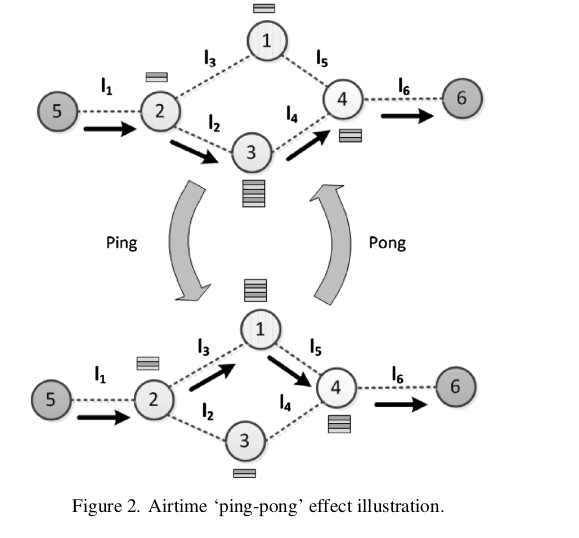
\includegraphics[width=.7\textwidth]{resources/img/chap5/message_exchange}
%					\caption{``\textit{Open LoRa Mesh}'' architecture}
%					\label{img:openmesh_architecture}
%				\end{figure}
			
			\subsubsection{Loop}
			
			\subsubsection{Listen}
			
			\subsubsection{Message forwarding}
			
			\subsubsection{MegaSense communication}
			
			\subsubsection{Message transmission}
			
		\subsection{Supported messages}
		
	\section{Other files}
	
%		\begin{figure}[h]
%			\centering
%			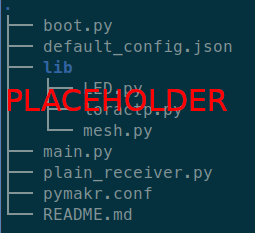
\includegraphics[width=.5\textwidth]{resources/img/chap5/tree_files}
%			\caption{List of files that compose the Open LoRa Mesh project}
%			\label{img:files}
%		\end{figure}
		
	\section{Microcontroller sleep cycle}\label{sec:sleep}
	
		Most IoT devices that compose LPWANs have three main modes, or profiles: \textit{sense}, \textit{connect} and \textit{sleep}.
		Sense and connect refer respectively to gathering data from the sensors and sending it into the network, while sleep refers to a sleep-mode energy consumption where most processes in the device are halted, and some circuits may be powered down.
		It can be considered a design trade-off between functionality, size, and battery lifetime.
		
		This energy consumption profile is important because it helps maximizing the battery life, which currently is one of the most considerable bottlenecks in IoT low-power devices, as explained in Section~\ref{sec:trends}.
		
		However, in the implementation of the Open LoRa Mesh, nodes do not have such functionality implemented, since might it be the cause for network disruptions.
		
		For example, if a new node might want to join a network, but the nearest physical node is in sleep mode, there would be no possibility for the new node to request data about the network, thus wasting time and resources while waiting to the other node to come back online.
		
		Such mode could be implemented but would require an careful analysis on the evolution of the network in time, also would require a network made entirely, or mostly of static nodes.
		This thought is reviewed again in Section~\ref{sec:software_improvements}.
			
	\section{Use cases}
		
		\subsection{Mobile network}
		
			e.g. in a bike sharing environment
		
		\subsection{Fixed network}
		
			e.g. in a monitoring values of air quality inside a building
		
		\subsection{Hybrid network}
		
			e.g. integrating mobile sensors given to users with a network of fixed sensors